\section{Jeu Loopy}

Le jeu \textit{Loopy} se joue sur une grille composée de cases et d'arêtes. Le but est de sélectionner certaines arêtes de la grille afin de former une unique boucle fermée.

Certaines cases contiennent un indice numérique. Cet indice indique exactement combien d'arêtes du contour de la case doivent appartenir à la boucle. Les cases sans indice n'imposent aucune contrainte directe sur le nombre d'arêtes sélectionnées autour d'elles.

Une solution valide doit donc vérifier trois conditions principales :
\begin{itemize}
    \item chaque case numérotée doit respecter son indice ;
    \item les arêtes sélectionnées doivent former une ou plusieurs courbes fermées, sans extrémité libre ni branchement ;
    \item il doit exister une seule boucle globale.
\end{itemize}

Les deux premières conditions sont locales et peuvent être modélisées directement par des contraintes linéaires. En revanche, la dernière condition est globale : elle impose l'unicité de la boucle. C'est cette règle qui rend le problème plus difficile à modéliser directement.

\subsection{Modélisation PLNE}

\subsubsection{Ensembles et paramètres}

On considère une grille rectangulaire composée de cases carrées. On introduit les ensembles et paramètres suivants :
\begin{itemize}
    \item \(\mathcal{E}\) : ensemble de toutes les arêtes de la grille ;
    \item \(\mathcal{V}\) : ensemble de tous les sommets de la grille ;
    \item \(\mathcal{S}\) : ensemble des cases portant un indice ;
    \item pour toute case \(p \in \mathcal{S}\), \(E(p) \subseteq \mathcal{E}\) désigne l'ensemble des quatre arêtes bordant la case \(p\) ;
    \item pour tout sommet \(v \in \mathcal{V}\), \(\delta(v) \subseteq \mathcal{E}\) désigne l'ensemble des arêtes incidentes au sommet \(v\) ;
    \item pour toute case \(p \in \mathcal{S}\), \(a_p \in \{0,1,2,3\}\) représente l'indice inscrit dans la case.
\end{itemize}

\subsubsection{Variables}

Pour chaque arête \(e \in \mathcal{E}\), on introduit une variable binaire :
\[
x_e =
\begin{cases}
1 & \text{si l'arête } e \text{ appartient à la boucle},\\
0 & \text{sinon}.
\end{cases}
\]

Afin d'imposer qu'un sommet soit soit absent de la boucle, soit traversé par la boucle, on introduit également une variable binaire pour chaque sommet \(v \in \mathcal{V}\) :
\[
y_v =
\begin{cases}
1 & \text{si le sommet } v \text{ appartient à la boucle},\\
0 & \text{sinon}.
\end{cases}
\]

\subsubsection{Contraintes des cases}

Chaque case numérotée doit être bordée par exactement le nombre d'arêtes indiqué par son indice. On impose donc :
\[
\sum_{e \in E(p)} x_e = a_p
\qquad \forall p \in \mathcal{S}.
\]

Cette contrainte garantit le respect des indices donnés dans la grille.

\subsubsection{Contraintes des sommets}

Dans une boucle, un sommet ne peut pas être une extrémité libre ni un point de branchement. Il doit donc être incident à exactement deux arêtes sélectionnées s'il appartient à la boucle, et à aucune arête sinon. On impose :
\[
\sum_{e \in \delta(v)} x_e = 2y_v
\qquad \forall v \in \mathcal{V}.
\]

Les variables sont binaires :
\[
x_e \in \{0,1\}
\qquad \forall e \in \mathcal{E},
\]
\[
y_v \in \{0,1\}
\qquad \forall v \in \mathcal{V}.
\]

Ces contraintes garantissent que les arêtes sélectionnées forment un ensemble de cycles disjoints, sans branchement et sans extrémité libre.

\subsubsection{Fonction objectif}

Le jeu \textit{Loopy} est formulé comme un problème de faisabilité. L'objectif n'est donc pas de minimiser ou maximiser une quantité particulière, mais simplement de trouver une solution réalisable. On choisit alors une fonction objectif constante :
\[
\min 0.
\]

Le modèle de base s'écrit donc :
\[
\min 0
\]
sous les contraintes :
\[
\sum_{e \in E(p)} x_e = a_p
\qquad \forall p \in \mathcal{S},
\]
\[
\sum_{e \in \delta(v)} x_e = 2y_v
\qquad \forall v \in \mathcal{V},
\]
\[
x_e \in \{0,1\}
\qquad \forall e \in \mathcal{E},
\]
\[
y_v \in \{0,1\}
\qquad \forall v \in \mathcal{V}.
\]

\subsubsection{Limite du modèle}

Le modèle précédent impose correctement les contraintes locales du jeu : les indices des cases sont respectés et les sommets sélectionnés sont de degré deux. Cependant, il ne garantit pas que toutes les arêtes sélectionnées appartiennent à une unique boucle.

En effet, le modèle peut produire plusieurs cycles disjoints. Une telle solution respecte les contraintes sur les cases et les sommets, mais elle n'est pas valide pour le jeu \textit{Loopy}, car la règle impose une seule boucle fermée.

Une formulation théorique possible consisterait à interdire tous les sous-cycles. Pour tout sous-ensemble strict non vide de sommets \(W \subset \mathcal{V}\), on pourrait ajouter une contrainte du type :
\[
\sum_{e \in E(W)} x_e \leq |W| - 1,
\qquad
\forall W \subset \mathcal{V}, \quad 2 \leq |W| < |\mathcal{V}|,
\]
où \(E(W)\) désigne l'ensemble des arêtes dont les deux extrémités appartiennent à \(W\).

Cependant, le nombre de ces contraintes est exponentiel par rapport au nombre de sommets. Il n'est donc pas raisonnable de les ajouter toutes dès le début de la résolution. Pour cette raison, la contrainte d'unicité de la boucle est traitée dynamiquement à l'aide d'un callback.

\subsection{Callback}

\subsubsection{Problème des sous-cycles}

La principale difficulté du jeu \textit{Loopy} est d'imposer que la solution contienne une seule boucle. Les contraintes locales du modèle PLNE empêchent les extrémités libres et les branchements, mais elles n'empêchent pas l'apparition de plusieurs cycles séparés.

Ainsi, une solution entière trouvée par CPLEX peut être localement correcte, tout en étant globalement invalide. Le rôle du callback est donc de tester chaque solution entière candidate et d'ajouter une contrainte supplémentaire lorsqu'une sous-boucle est détectée.

\subsubsection{Détection des composantes connexes}

Lorsqu'une solution entière est trouvée par CPLEX, on récupère l'ensemble des arêtes sélectionnées :
\[
\{e \in \mathcal{E} \mid x_e = 1\}.
\]

À partir de ces arêtes, on construit le graphe correspondant, dont les sommets sont les sommets de la grille et dont les arêtes sont les arêtes sélectionnées. On recherche ensuite les composantes connexes de ce graphe.

Si toutes les arêtes sélectionnées appartiennent à une seule composante connexe, alors la solution contient une unique boucle et elle est acceptée. En revanche, si plusieurs composantes connexes sont détectées, cela signifie que la solution contient plusieurs boucles disjointes. Dans ce cas, la solution doit être rejetée.

\subsubsection{Contrainte ajoutée}

Lorsqu'une sous-boucle est détectée, on note \(C\) l'ensemble des arêtes de cette boucle. Pour interdire à CPLEX de retrouver exactement cette même sous-boucle, on ajoute dynamiquement la contrainte suivante :
\[
\sum_{e \in C} x_e \leq |C| - 1.
\]

Cette contrainte force au moins une arête de la sous-boucle \(C\) à ne plus être sélectionnée. La solution courante est donc éliminée, et CPLEX poursuit la résolution avec cette nouvelle contrainte.

Le callback suit alors le principe suivant :
\begin{enumerate}
    \item CPLEX trouve une solution entière candidate ;
    \item on récupère les arêtes telles que \(x_e = 1\) ;
    \item on construit le graphe associé aux arêtes sélectionnées ;
    \item on calcule les composantes connexes de ce graphe ;
    \item si une seule composante est présente, la solution est acceptée ;
    \item sinon, on ajoute une contrainte de coupe sur une sous-boucle détectée.
\end{enumerate}

Cette approche permet de ne pas ajouter toutes les contraintes d'unicité dès le début. Les contraintes sont ajoutées uniquement lorsqu'elles sont nécessaires, ce qui rend la résolution plus efficace pour les instances de taille raisonnable.

\subsubsection{Définition manuelle d’une instance}

On crée dans le répertoire \texttt{data} un fichier \texttt{instanceTest.txt} représentant une instance simple du jeu \textit{Loopy}. 

Dans ce jeu, une instance est définie par une grille contenant :
\begin{itemize}
    \item des entiers entre 0 et 3 indiquant le nombre d’arêtes à sélectionner autour d’une case ;
    \item des cases vides (sans contrainte).
\end{itemize}

Nous adoptons un format texte simple où :
\begin{itemize}
    \item chaque ligne correspond à une ligne de la grille ;
    \item les valeurs sont séparées par des virgules ;
    \item une case vide est représentée par un espace.
\end{itemize}

\subsubsection{Exemple d’instance}

Considérons une grille \(4 \times 4\) :

\begin{center}
\ttfamily
\begin{tabular}{cccc}
 , & 2, & 3, &  \\
 1, &  , &  , & 2 \\
 , & 3, &  , &  \\
 2, &  , & 1, &  
\end{tabular}
\end{center}



\subsubsection{Interprétation}

\begin{itemize}
    \item La case \((1,2)\) contient la valeur 2 : exactement 2 arêtes autour de cette case doivent appartenir à la boucle.
    \item La case \((2,1)\) contient la valeur 1 : une seule arête doit être sélectionnée.
    \item Les cases vides n’imposent aucune contrainte.
\end{itemize}

Cette instance sera utilisée pour tester la lecture des données et la résolution du modèle.

\subsection{Implémentation}

Cette section présente les principales fonctions développées pour manipuler les instances du jeu \textit{Loopy}. L'implémentation est organisée autour de trois aspects : la lecture des instances, l'affichage des grilles et la génération automatique d'instances de test.

\subsubsection{Lecture des instances}

Les instances du jeu \textit{Loopy} sont représentées par une matrice d'entiers. Chaque case de la grille correspond à une valeur :
\begin{itemize}
    \item une valeur entre \(0\) et \(3\) représente une case contenant un indice ;
    \item la valeur \(-1\) représente une case vide, c'est-à-dire une case sans contrainte.
\end{itemize}

Le fichier d'entrée est un fichier texte dans lequel chaque ligne correspond à une ligne de la grille. Les valeurs sont séparées par des virgules, et une case vide est représentée par un espace. Par exemple :
\[
\texttt{1, ,3, ,2}
\]

La fonction \texttt{readInputFile} lit le fichier ligne par ligne, sépare les valeurs selon les virgules, puis construit la matrice associée. Les cases vides sont détectées après suppression des espaces et sont remplacées par la valeur \(-1\).

\begin{verbatim}
if val == ""
    grid[i, j] = -1
else
    grid[i, j] = parse(Int64, val)
end
\end{verbatim}

Ainsi, une instance textuelle peut être directement convertie en une structure exploitable par le modèle de résolution.

\subsubsection{Affichage}

Deux fonctions d'affichage ont été ajoutées dans le fichier \texttt{io.jl}. La première, \texttt{displayGrid}, affiche une instance non résolue dans la console. Les cases vides sont représentées par un point, tandis que les cases numérotées affichent leur indice.

La deuxième fonction, \texttt{displaySolution}, affiche une solution obtenue par CPLEX. Elle prend en entrée les variables correspondant aux arêtes horizontales et verticales. Après récupération des valeurs numériques avec \texttt{JuMP.value}, les arêtes sélectionnées sont affichées dans la console.

Les arêtes horizontales sélectionnées sont représentées par \texttt{---}, tandis que les arêtes verticales sélectionnées sont représentées par \texttt{|}. Une arête est considérée comme sélectionnée lorsque sa valeur est supérieure à \(0.5\).

\begin{verbatim}
if hVal[i, j] > 0.5
    print("---")
else
    print("   ")
end
\end{verbatim}

Cette représentation permet de vérifier rapidement la forme de la boucle obtenue.

\begin{figure}[H]
    \centering
    \begin{minipage}{0.42\textwidth}
        \centering
        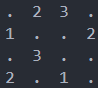
\includegraphics[width=\linewidth,height=4.5cm,keepaspectratio]{imgs/loopy_instance.png}
        \\
        \small Instance
    \end{minipage}
    \hspace{0.05\textwidth}
    \begin{minipage}{0.42\textwidth}
        \centering
        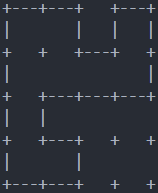
\includegraphics[width=\linewidth,height=4.5cm,keepaspectratio]{imgs/loopy_solution.png}
        \\
        \small Solution
    \end{minipage}
    \caption{Affichage en ligne de commande d'une instance et d'une solution \textit{Loopy}.}
\end{figure}

\subsection{Génération des instances}

Afin de tester le modèle sur plusieurs types de grilles, nous avons implémenté une fonction \texttt{generateInstance}. Cette fonction génère une grille aléatoire de taille donnée. Le paramètre \texttt{density} contrôle la proportion approximative de cases contenant un indice.

Chaque case est initialement vide, donc égale à \(-1\). Ensuite, pour chaque case, un indice est ajouté avec une probabilité égale à \texttt{density}. Si un indice est ajouté, sa valeur est choisie aléatoirement entre \(0\) et \(3\).

\begin{verbatim}
if rand() <= density
    grid[i, j] = rand(0:3)
end
\end{verbatim}

Nous avons ensuite défini une fonction \texttt{generateDataSet}, qui génère automatiquement plusieurs instances pour différentes tailles et densités. Les tailles considérées sont :
\[
4 \times 4,\quad 5 \times 5,\quad 6 \times 6,\quad 7 \times 7,\quad 8 \times 8.
\]

Les densités testées sont :
\[
0.20,\quad 0.30,\quad 0.40.
\]

Pour chaque couple taille-densité, cinq instances sont générées et enregistrées dans le dossier \texttt{data}. Les fichiers obtenus suivent une convention de nommage indiquant la taille, la densité et le numéro de l'instance, par exemple :
\[
\texttt{generated\_6x6\_d0.3\_2.txt}.
\]

Les instances générées ne sont pas nécessairement toutes réalisables, car les indices sont placés aléatoirement. Cela permet néanmoins de tester le comportement du modèle sur des instances variées, avec différentes tailles et différents niveaux de contrainte.

\subsection{Sauvegarde des instances}

La fonction \texttt{saveInstance} permet d'écrire une grille dans un fichier texte. Elle utilise le même format que celui attendu par la fonction \texttt{readInputFile}. Les cases vides, représentées par \(-1\) dans le programme, sont écrites comme des espaces dans le fichier.

Ainsi, une instance générée automatiquement peut être immédiatement relue par le programme puis utilisée par le modèle de résolution. Cette cohérence entre lecture et écriture facilite la génération de jeux de tests pour les expériences numériques.

\subsection{Implémentation du modèle}

\subsubsection{Méthode \texttt{cplexSolve}}

Le modèle est implémenté à l'aide du solveur CPLEX via la bibliothèque \texttt{JuMP}. La méthode \texttt{cplexSolve} prend en entrée une matrice représentant la grille du jeu et retourne :
\begin{itemize}
    \item un booléen indiquant si une solution réalisable est trouvée ;
    \item le temps de résolution ;
    \item les variables représentant la solution, c'est-à-dire les arêtes horizontales et verticales sélectionnées.
\end{itemize}

\subsubsection{Variables}

Pour une grille de taille \(n \times m\), on introduit :
\begin{itemize}
    \item \(h_{i,j} \in \{0,1\}\) : vaut 1 si l'arête horizontale \((i,j)\) est sélectionnée ;
    \item \(v_{i,j} \in \{0,1\}\) : vaut 1 si l'arête verticale \((i,j)\) est sélectionnée ;
    \item \(y_{i,j} \in \{0,1\}\) : vaut 1 si le sommet \((i,j)\) appartient à la boucle.
\end{itemize}

\subsubsection{Fonction objectif}

On cherche uniquement une solution réalisable :
\[
\min 0
\]

\subsubsection{Contraintes}

\paragraph{Contraintes sur les cases}
Pour chaque case numérotée \((i,j)\), la somme des quatre arêtes qui l'entourent doit être égale à l'indice de la case :
\[
h_{i,j} + h_{i+1,j} + v_{i,j} + v_{i,j+1} = t_{i,j}.
\]

\paragraph{Contraintes sur les sommets}
Chaque sommet doit avoir un degré égal à 0 ou 2 :
\[
\sum_{e \in \delta(i,j)} x_e = 2y_{i,j}.
\]

\subsubsection{Test de la méthode}

La méthode a été testée sur l'instance \texttt{data/instanceTest.txt}. Après lecture de l'instance par la méthode \texttt{readInputFile}, la commande suivante a été exécutée :
\begin{verbatim}
isFeasible, solveTime, h, v = cplexSolve(grid)
\end{verbatim}

Le solveur CPLEX trouve une solution réalisable :
\begin{verbatim}
Solution trouvée : true
Temps : 0.013 s
\end{verbatim}

Ainsi, le modèle de base permet bien de résoudre l'instance test et de retourner les variables représentant les arêtes horizontales et verticales de la solution.

\subsubsection{Remarque}

Ce modèle garantit que les arêtes sélectionnées respectent les contraintes locales des cases et forment une union de cycles sans branchement. Toutefois, il n'impose pas encore que la solution soit une unique boucle. Cette contrainte sera traitée à l'aide d'un callback.

\subsubsection{Traitement de la règle difficile par callback}

La règle difficile du jeu \textit{Loopy} est l'unicité de la boucle. En effet, les contraintes du modèle de base imposent seulement que chaque sommet ait un degré égal à 0 ou 2. Elles garantissent donc l'absence de branchements, mais elles peuvent encore autoriser plusieurs cycles disjoints.

Afin de corriger ce problème, nous utilisons un callback CPLEX. À chaque fois que CPLEX trouve une solution entière, le callback récupère les arêtes sélectionnées, reconstruit les composantes connexes formées par ces arêtes, puis vérifie si plusieurs cycles sont présents.

Si plusieurs composantes sont détectées, alors la solution ne respecte pas la règle du jeu. Pour chaque sous-boucle \(C\), on ajoute dynamiquement la contrainte suivante :
\[
\sum_{e \in C} x_e \leq |C|-1.
\]

Cette contrainte interdit à la même sous-boucle de réapparaître dans une solution future. Ainsi, CPLEX poursuit la résolution jusqu'à trouver une solution constituée d'une seule boucle.

Le callback suit donc les étapes suivantes :
\begin{enumerate}
    \item récupérer la solution entière courante ;
    \item identifier les arêtes sélectionnées ;
    \item construire les composantes connexes ;
    \item si plusieurs boucles sont présentes, ajouter une contrainte de coupe ;
    \item continuer la résolution.
\end{enumerate}

\subsubsection{Test du callback}

La méthode \texttt{cplexSolveWithCallback} a été testée sur l'instance \texttt{data/instanceTest.txt}. Le callback est bien activé par CPLEX, comme l'indique l'affichage :
\begin{verbatim}
CPXPARAM_Threads 1
Generic callback
\end{verbatim}

La résolution retourne :
\begin{verbatim}
Solution trouvée : true
Temps : 2.19 s
\end{verbatim}

Ainsi, le modèle avec callback permet de trouver une solution réalisable tout en prenant en compte la contrainte difficile d'unicité de la boucle.

Cette approche évite d'ajouter dès le départ toutes les contraintes d'élimination de sous-boucles, qui seraient trop nombreuses.

\subsection{Résolution de plusieurs instances}

Afin d'évaluer les performances des méthodes de résolution, nous avons implémenté une fonction \texttt{solveDataSet}. Cette fonction permet de résoudre automatiquement toutes les instances contenues dans le dossier \texttt{data}.

Pour chaque fichier d'instance, la grille est d'abord lue à l'aide de la fonction \texttt{readInputFile}. Ensuite, deux méthodes de résolution sont appliquées :
\begin{itemize}
    \item la résolution exacte par CPLEX avec callback ;
    \item une résolution heuristique.
\end{itemize}

Les résultats sont enregistrés séparément dans deux sous-dossiers :
\[
\texttt{res/cplex}
\qquad \text{et} \qquad
\texttt{res/heuristique}.
\]

Pour chaque instance et pour chaque méthode, un fichier de résultat est créé. Ce fichier contient au minimum deux informations :
\begin{itemize}
    \item \texttt{solveTime} : le temps de résolution ;
    \item \texttt{isOptimal} : un booléen indiquant si une solution a été trouvée.
\end{itemize}

Si une solution est trouvée, les valeurs des arêtes horizontales et verticales sont également sauvegardées dans le fichier de sortie. Cela permet de conserver la solution obtenue et de l'afficher ensuite si nécessaire.

Le principe général de la fonction est le suivant :
\begin{enumerate}
    \item parcourir tous les fichiers du dossier \texttt{data} ;
    \item lire chaque instance ;
    \item résoudre l'instance avec CPLEX et avec l'heuristique ;
    \item sauvegarder les résultats dans le dossier correspondant ;
    \item afficher dans la console le statut de résolution et le temps obtenu.
\end{enumerate}

Un extrait représentatif de cette procédure est donné ci-dessous :

\begin{verbatim}
for file in filter(x -> occursin(".txt", x), readdir(dataFolder))

    grid = readInputFile(dataFolder * file)

    for method in resolutionMethod

        if method == "cplex"
            isOptimal, solveTime, h, v = cplexSolveWithCallback(grid)
        else
            isOptimal, solveTime, h, v = heuristicSolve(grid)
        end

        println(fout, "solveTime = ", solveTime)
        println(fout, "isOptimal = ", isOptimal)
    end
end
\end{verbatim}

Cette organisation permet ensuite d'exploiter automatiquement les fichiers de résultats pour construire des tableaux comparatifs et analyser les performances des méthodes selon la taille et la densité des instances.

\subsection{Méthode heuristique}

En plus de la résolution exacte par CPLEX, nous avons implémenté une méthode heuristique pour tenter de trouver rapidement une solution réalisable. Contrairement à la méthode exacte, cette approche ne garantit pas toujours de trouver une solution, même si une solution existe. Elle permet cependant d'obtenir rapidement une configuration satisfaisante sur certaines instances.

\subsubsection{Principe général}

L'heuristique repose sur une recherche locale. On représente une solution candidate à l'aide de deux matrices binaires :
\begin{itemize}
    \item \(h\), qui représente les arêtes horizontales sélectionnées ;
    \item \(v\), qui représente les arêtes verticales sélectionnées.
\end{itemize}

Une valeur égale à \(1\) signifie que l'arête est sélectionnée, tandis qu'une valeur égale à \(0\) signifie qu'elle ne l'est pas.

L'algorithme commence par générer aléatoirement une configuration initiale des arêtes. Ensuite, il modifie progressivement cette configuration en inversant l'état d'une arête choisie au hasard. À chaque modification, une fonction de score permet d'évaluer la qualité de la solution obtenue.

\subsubsection{Fonction de score}

La fonction de score mesure le nombre de violations des contraintes locales du jeu. Elle prend en compte deux types de pénalités.

D'abord, pour chaque case numérotée, on compare le nombre d'arêtes sélectionnées autour de cette case avec l'indice demandé. Si la case \(p\) porte l'indice \(a_p\), on ajoute au score l'écart :
\[
\left| \sum_{e \in E(p)} x_e - a_p \right|.
\]

Ensuite, on vérifie les degrés des sommets. Dans une boucle valide, chaque sommet doit avoir un degré égal à \(0\) ou à \(2\). Si un sommet a un degré différent, une pénalité est ajoutée au score.

Ainsi, plus le score est faible, plus la configuration est proche d'une solution valide. Un score nul signifie que toutes les contraintes locales sont satisfaites.

Un extrait représentatif de cette fonction est donné ci-dessous :
\begin{verbatim}
if t[i,j] != -1
    s = h[i,j] + h[i+1,j] + v[i,j] + v[i,j+1]
    score += abs(s - t[i,j])
end
\end{verbatim}

Cette partie du code calcule, pour chaque case numérotée, le nombre d'arêtes sélectionnées autour de la case et le compare avec l'indice imposé.

\subsubsection{Recherche locale}

À chaque itération, l'heuristique crée une nouvelle solution candidate à partir de la meilleure solution courante. Pour cela, elle choisit aléatoirement une arête horizontale ou verticale, puis inverse son état.

Si la nouvelle solution possède un score inférieur ou égal au meilleur score courant, elle est acceptée. Afin d'éviter de rester bloqué dans un minimum local, l'algorithme accepte également, avec une faible probabilité, une solution légèrement moins bonne.

\begin{verbatim}
if newScore <= bestScore || rand() < 0.01
    bestH = h2
    bestV = v2
    bestScore = newScore
end
\end{verbatim}

Cette stratégie permet d'explorer plusieurs configurations possibles au lieu de suivre uniquement les améliorations immédiates.

\subsubsection{Critère d'arrêt}

L'algorithme s'arrête lorsque l'une des deux conditions suivantes est vérifiée :
\begin{itemize}
    \item une configuration de score nul est trouvée ;
    \item la limite de temps fixée est atteinte.
\end{itemize}

Dans notre implémentation, la limite de temps par défaut est fixée à \(20\) secondes. À la fin de l'exécution, la fonction retourne :
\begin{itemize}
    \item un booléen indiquant si une configuration de score nul a été trouvée ;
    \item le temps de calcul ;
    \item les matrices \(h\) et \(v\) correspondant à la meilleure solution trouvée.
\end{itemize}

\subsubsection{Limites de l'heuristique}

Cette heuristique est simple et rapide, mais elle présente certaines limites. Elle se base principalement sur les contraintes locales : les indices des cases et les degrés des sommets. Elle permet donc de réduire progressivement les violations locales, mais elle ne garantit pas toujours l'obtention d'une unique boucle globale.

En particulier, une configuration peut avoir un score nul pour les contraintes locales tout en contenant plusieurs cycles disjoints. Cette difficulté est précisément celle qui justifie l'utilisation du callback dans la méthode exacte.

Ainsi, l'heuristique constitue surtout une méthode approchée permettant de trouver rapidement de bonnes configurations, tandis que la résolution exacte avec callback reste nécessaire pour garantir rigoureusement la validité complète d'une solution du jeu \textit{Loopy}.

\subsection{Résultats expérimentaux}

\subsubsection{Protocole}

Les expériences ont été réalisées sur des instances générées automatiquement. Les tailles de grilles testées sont :
\[
4 \times 4,\quad 5 \times 5,\quad 6 \times 6,\quad 7 \times 7,\quad 8 \times 8.
\]

Pour chaque taille, trois densités d'indices ont été considérées :
\[
0.20,\quad 0.30,\quad 0.40.
\]

Pour chaque couple taille-densité, cinq instances ont été générées. Cela donne donc :
\[
5 \text{ tailles} \times 3 \text{ densités} \times 5 \text{ instances}
= 75 \text{ instances}.
\]

Une instance manuelle, \texttt{instanceTest.txt}, a également été utilisée pour vérifier le bon fonctionnement du modèle sur un cas simple.

Deux méthodes de résolution ont été comparées :
\begin{itemize}
    \item une résolution exacte par CPLEX avec callback ;
    \item une résolution heuristique basée sur une recherche locale.
\end{itemize}

Pour chaque instance et chaque méthode, nous avons enregistré le temps de calcul \texttt{solveTime} ainsi que la variable \texttt{isOptimal}, qui indique si une solution a été trouvée. Pour l'heuristique, la limite de temps est fixée à \(20\) secondes par instance.

\subsubsection{Temps de calcul}

Le tableau suivant présente les temps moyens de calcul par taille de grille. Les moyennes sont calculées sur les \(15\) instances générées pour chaque taille, toutes densités confondues.

\begin{center}
\renewcommand{\arraystretch}{1.2}
\begin{tabular}{c|c|c}
\hline
\textbf{Taille} & \textbf{Temps moyen CPLEX (s)} & \textbf{Temps moyen heuristique (s)} \\
\hline
\(4 \times 4\) & 0.167 & 9.337 \\
\(5 \times 5\) & 0.004 & 14.676 \\
\(6 \times 6\) & 0.005 & 12.096 \\
\(7 \times 7\) & 0.009 & 13.747 \\
\(8 \times 8\) & 0.002 & 19.370 \\
\hline
\end{tabular}
\end{center}

On remarque que CPLEX retourne une réponse très rapidement sur la majorité des instances. Les temps moyens restent très faibles pour toutes les tailles testées. Le temps moyen le plus élevé est observé pour les instances de taille \(4 \times 4\), principalement à cause d'une instance résolue en \(2.29\) secondes. Pour les autres tailles, les temps moyens restent proches de zéro.

Pour l'heuristique, les temps moyens sont nettement plus élevés. Cela s'explique par le fait que l'heuristique atteint souvent sa limite de temps de \(20\) secondes lorsqu'elle ne trouve pas de solution. En revanche, lorsqu'une solution est trouvée, le temps peut être faible, parfois inférieur à une seconde.

Ces résultats montrent donc que, sur les instances testées, le modèle PLNE avec CPLEX est très rapide pour conclure, alors que l'heuristique est plus irrégulière : elle peut trouver certaines solutions rapidement, mais elle peut aussi échouer et atteindre la limite de temps.

\begin{figure}[H]
\centering
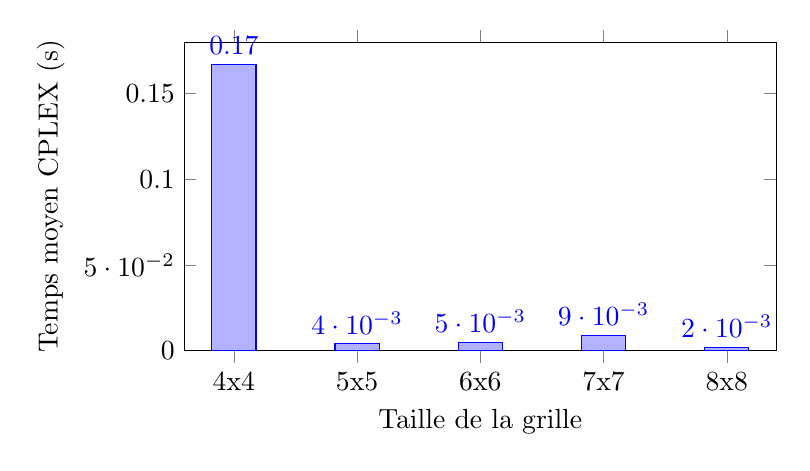
\begin{tikzpicture}
\begin{axis}[
    ybar,
    width=0.75\textwidth,
    height=5.5cm,
    bar width=16pt,
    ylabel={Temps moyen CPLEX (s)},
    xlabel={Taille de la grille},
    symbolic x coords={4x4,5x5,6x6,7x7,8x8},
    xtick=data,
    ymin=0,
    ymax=0.18,
    nodes near coords,
    nodes near coords align={vertical},
]
\addplot coordinates {
    (4x4,0.167)
    (5x5,0.004)
    (6x6,0.005)
    (7x7,0.009)
    (8x8,0.002)
};
\end{axis}
\end{tikzpicture}
\caption{Temps moyen de résolution avec CPLEX selon la taille de la grille.}
\end{figure}

\begin{figure}[H]
\centering
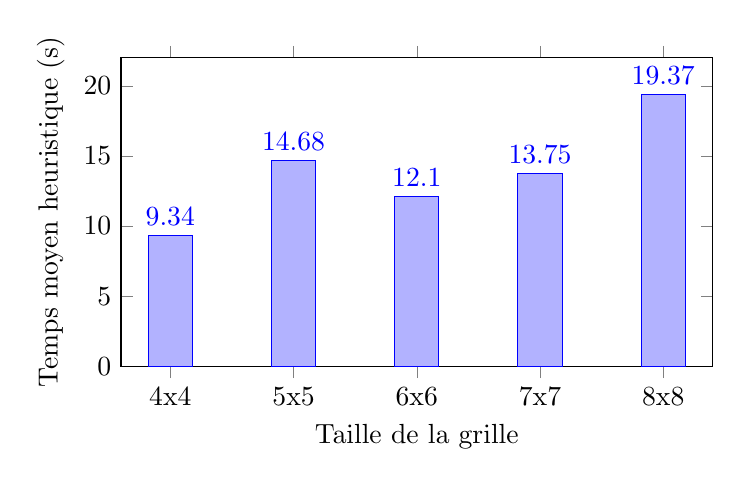
\begin{tikzpicture}
\begin{axis}[
    ybar,
    width=0.75\textwidth,
    height=5.5cm,
    bar width=16pt,
    ylabel={Temps moyen heuristique (s)},
    xlabel={Taille de la grille},
    symbolic x coords={4x4,5x5,6x6,7x7,8x8},
    xtick=data,
    ymin=0,
    ymax=22,
    nodes near coords,
    nodes near coords align={vertical},
]
\addplot coordinates {
    (4x4,9.337)
    (5x5,14.676)
    (6x6,12.096)
    (7x7,13.747)
    (8x8,19.370)
};
\end{axis}
\end{tikzpicture}
\caption{Temps moyen de résolution avec l'heuristique selon la taille de la grille.}
\end{figure}


\subsubsection{Taux de résolution}

Le tableau suivant présente le nombre d'instances résolues par chaque méthode, regroupé par taille de grille. On considère ici les \(15\) instances générées pour chaque taille, toutes densités confondues.

\begin{center}
\renewcommand{\arraystretch}{1.2}
\begin{tabular}{c|c|c|c}
\hline
\textbf{Taille} & \textbf{Nb. instances} & \textbf{CPLEX résolues} & \textbf{Heuristique résolues} \\
\hline
\(4 \times 4\) & 15 & 8 & 8 \\
\(5 \times 5\) & 15 & 4 & 4 \\
\(6 \times 6\) & 15 & 6 & 6 \\
\(7 \times 7\) & 15 & 6 & 5 \\
\(8 \times 8\) & 15 & 1 & 1 \\
\hline
\textbf{Total} & \textbf{75} & \textbf{25} & \textbf{24} \\
\hline
\end{tabular}
\end{center}

Les taux de résolution globaux sur les instances générées sont donc :
\[
\text{Taux CPLEX} = \frac{25}{75} \approx 33.3\%,
\]
\[
\text{Taux heuristique} = \frac{24}{75} = 32.0\%.
\]


\begin{figure}[H]
\centering
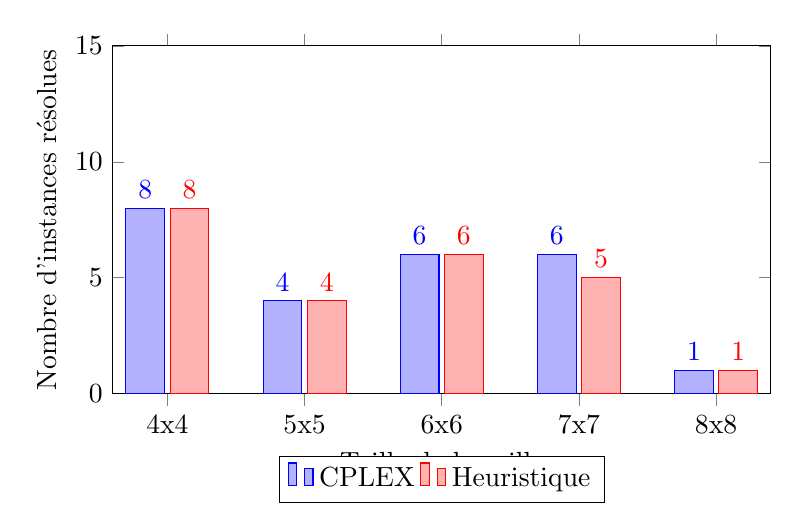
\begin{tikzpicture}
\begin{axis}[
    ybar,
    width=0.82\textwidth,
    height=6cm,
    bar width=14pt,
    ylabel={Nombre d'instances résolues},
    xlabel={Taille de la grille},
    symbolic x coords={4x4,5x5,6x6,7x7,8x8},
    xtick=data,
    ymin=0,
    ymax=15,
    legend style={at={(0.5,-0.18)},anchor=north,legend columns=2},
    nodes near coords,
    nodes near coords align={vertical},
]
\addplot coordinates {(4x4,8) (5x5,4) (6x6,6) (7x7,6) (8x8,1)};
\addplot coordinates {(4x4,8) (5x5,4) (6x6,6) (7x7,5) (8x8,1)};
\legend{CPLEX, Heuristique}
\end{axis}
\end{tikzpicture}
\caption{Nombre d'instances résolues par taille de grille.}
\end{figure}

On observe que les deux méthodes obtiennent des taux de résolution assez proches sur l'ensemble des instances générées. CPLEX résout \(25\) instances, tandis que l'heuristique en résout \(24\). La différence principale entre les deux méthodes n'est donc pas seulement le nombre d'instances résolues, mais aussi le temps nécessaire pour conclure.

En effet, CPLEX retourne souvent une réponse très rapidement, que l'instance soit réalisable ou non. L'heuristique, au contraire, peut trouver certaines solutions rapidement, mais atteint souvent la limite de temps lorsqu'elle ne parvient pas à construire une solution valide.

On remarque également que les instances de taille \(8 \times 8\) sont beaucoup plus difficiles : une seule instance est résolue par chaque méthode. Cela est cohérent avec l'augmentation du nombre d'arêtes, de sommets et donc de la taille de l'espace de recherche.

Enfin, il faut noter que les instances sont générées aléatoirement et ne sont pas nécessairement réalisables. Ainsi, lorsqu'aucune solution n'est trouvée, cela ne signifie pas forcément que la méthode échoue : l'instance peut aussi être infaisable.

\subsubsection{Taille maximale résolue}

D'après les résultats obtenus, la méthode exacte par CPLEX avec callback trouve des solutions jusqu'à la taille \(8 \times 8\). En effet, une instance générée de taille \(8 \times 8\) a été résolue par CPLEX dans notre série de tests.

L'heuristique trouve également au moins une solution jusqu'à la taille \(8 \times 8\). Cependant, ce résultat doit être interprété avec prudence. En effet, l'heuristique repose principalement sur une fonction de score qui pénalise les violations des contraintes locales : respect des indices et degrés des sommets. Elle permet donc de trouver rapidement de bonnes configurations candidates, mais elle ne garantit pas systématiquement l'unicité globale de la boucle.

Ainsi, pour obtenir une solution rigoureusement valide du jeu \textit{Loopy}, la méthode exacte avec callback reste la méthode la plus fiable. L'heuristique constitue plutôt une méthode complémentaire, utile pour explorer rapidement l'espace des solutions.

\subsubsection{Gap éventuel}

Dans notre modélisation, le jeu \textit{Loopy} est formulé comme un problème de faisabilité. La fonction objectif choisie est constante :
\[
\min 0.
\]

Il n'y a donc pas de véritable quantité à optimiser. Par conséquent, le calcul d'un gap relatif entre la meilleure relaxation linéaire et la meilleure solution entière connue n'est pas pertinent dans notre cas.

L'évaluation expérimentale repose donc principalement sur :
\begin{itemize}
    \item le temps de calcul ;
    \item le nombre d'instances résolues ;
    \item la taille maximale atteinte ;
    \item la capacité de la méthode à garantir l'unicité de la boucle.
\end{itemize}

\subsubsection{Bilan}

Les résultats montrent que la résolution exacte avec callback est très rapide sur les instances où elle conclut. Elle permet de résoudre certaines instances jusqu'à la taille \(8 \times 8\), tout en garantissant la validité complète de la solution, notamment l'unicité de la boucle.

L'heuristique obtient des résultats proches en nombre d'instances résolues, mais elle ne garantit pas toujours la contrainte globale d'unicité. Elle constitue donc une méthode complémentaire intéressante, mais moins rigoureuse que l'approche exacte.

Enfin, la difficulté augmente avec la taille des grilles et avec la structure des indices. Les instances générées aléatoirement peuvent également être infaisables, ce qui explique en partie les taux de résolution observés.

\subsection{Discussion}

Les résultats obtenus montrent que la résolution du jeu \textit{Loopy} dépend fortement de la structure des instances. Même pour des grilles de taille modérée, certaines instances deviennent difficiles à résoudre, notamment lorsque les indices imposent des contraintes fortes ou contradictoires.

La modélisation PLNE permet de représenter efficacement les contraintes locales du jeu. Les contraintes sur les cases numérotées assurent le respect des indices, tandis que les contraintes sur les sommets empêchent les extrémités libres et les branchements. Cependant, ces contraintes ne suffisent pas à garantir l'existence d'une unique boucle. Elles peuvent encore autoriser plusieurs cycles disjoints.

Le callback joue donc un rôle essentiel. Il permet de traiter dynamiquement la contrainte globale d'unicité de la boucle. Au lieu d'ajouter dès le départ un très grand nombre de contraintes interdisant toutes les sous-boucles possibles, le callback ajoute uniquement les contraintes nécessaires lorsqu'une solution entière invalide est détectée. Cette approche permet de garder un modèle initial plus léger.

La méthode exacte avec CPLEX présente l'avantage de fournir une validation rigoureuse des solutions obtenues. Lorsqu'une solution est retournée par le modèle avec callback, elle respecte à la fois les contraintes locales et la contrainte globale d'unicité de la boucle. En revanche, cette méthode peut devenir plus limitée lorsque la taille des instances augmente ou lorsque les instances générées sont difficiles.

L'heuristique, quant à elle, est plus simple à mettre en œuvre. Elle repose sur une recherche locale et sur une fonction de score pénalisant les violations des contraintes locales. Elle peut trouver rapidement certaines configurations intéressantes. Toutefois, elle ne garantit pas toujours l'unicité globale de la boucle : une solution satisfaisant les contraintes locales peut encore contenir plusieurs cycles disjoints.

Il faut également souligner que les instances générées aléatoirement ne sont pas nécessairement réalisables. Ainsi, lorsqu'une méthode ne trouve pas de solution, cela ne signifie pas forcément que la méthode échoue : l'instance peut simplement être infaisable. Pour obtenir une analyse plus précise, il serait intéressant de générer des instances à partir de solutions connues, puis de retirer progressivement certains indices.

Enfin, les résultats montrent que les deux approches sont complémentaires. La résolution exacte est plus fiable pour certifier une solution valide, tandis que l'heuristique peut servir à explorer rapidement l'espace des configurations et à obtenir des solutions candidates.

\subsection{Conclusion}

Dans ce projet, nous avons étudié la résolution automatique du jeu \textit{Loopy}. Nous avons d'abord proposé une modélisation du problème sous la forme d'un programme linéaire en nombres entiers. Cette modélisation repose sur des variables binaires associées aux arêtes de la grille, ainsi que sur des contraintes locales permettant de respecter les indices des cases et les degrés des sommets.

La principale difficulté du problème est la contrainte d'unicité de la boucle. En effet, les contraintes locales permettent seulement d'obtenir un ensemble de cycles disjoints, mais ne garantissent pas que toutes les arêtes sélectionnées forment une seule boucle. Pour traiter cette difficulté, nous avons utilisé un callback. Celui-ci détecte les sous-cycles dans les solutions entières proposées par CPLEX et ajoute dynamiquement des contraintes pour les interdire.

Nous avons également implémenté les fonctions nécessaires à la manipulation des instances : lecture depuis un fichier texte, affichage en console, génération automatique d'instances, résolution de plusieurs instances et sauvegarde des résultats. Une méthode heuristique basée sur une recherche locale a aussi été développée afin de comparer une approche approchée avec la résolution exacte.

Les expériences montrent que CPLEX avec callback fournit une méthode rigoureuse, capable de garantir la validité complète des solutions obtenues. Dans nos tests, cette méthode parvient à résoudre certaines instances jusqu'à la taille \(8 \times 8\). L'heuristique permet également de trouver des configurations candidates, mais elle ne garantit pas toujours l'unicité globale de la boucle.

Les résultats montrent aussi que la difficulté augmente avec la taille des grilles et que les instances générées aléatoirement peuvent être infaisables. Comme amélioration possible, on pourrait développer un générateur d'instances réalisables à partir de boucles connues. Cela permettrait de mieux comparer les méthodes sur des instances dont on sait qu'elles admettent au moins une solution. On pourrait également renforcer l'heuristique en ajoutant une vérification explicite de la connexité afin de mieux prendre en compte la contrainte globale du jeu.



\subsection{Annexes}

\subsubsection{Exemple d'instance}

Voici un exemple de fichier texte représentant une instance du jeu \textit{Loopy}. Les cases vides sont représentées par des espaces, tandis que les cases contraintes contiennent un entier entre \(0\) et \(3\).

\begin{verbatim}
 ,2, ,1
3, , , 
 , ,0, 
1, , ,2
\end{verbatim}

Après lecture par la fonction \texttt{readInputFile}, cette instance est transformée en matrice d'entiers. Les cases vides sont représentées par la valeur \(-1\).

\subsubsection{Exemple de solution sauvegardée}

Lorsqu'une solution est trouvée, les matrices des arêtes horizontales et verticales sont sauvegardées. La matrice \(h\) représente les arêtes horizontales et la matrice \(v\) représente les arêtes verticales.

\begin{verbatim}
h = [
1 0 1 0
0 1 0 1
1 0 0 1
0 1 1 0
1 0 1 0
]

v = [
1 0 1 0 1
0 1 0 1 0
1 0 0 1 0
0 1 1 0 1
]
\end{verbatim}

Une valeur \(1\) signifie que l'arête est sélectionnée, tandis qu'une valeur \(0\) signifie qu'elle ne l'est pas.

\subsubsection{Tableau détaillé des résultats}
\begin{center}
\scriptsize
\renewcommand{\arraystretch}{1.05}
\begin{tabular}{lrrrr}
\hline
\textbf{Instance} & \textbf{CPLEX t. (s)} & \textbf{CPLEX ok} & \textbf{Heur. t. (s)} & \textbf{Heur. ok} \\
\hline
generated\_4x4\_d0.2\_1.txt & 2.29 & 
$\times$
 & 0.0 & 
$\times$
\\
generated\_4x4\_d0.2\_2.txt & 0.0 & 
$\times$
 & 0.0 & 
$\times$
\\
generated\_4x4\_d0.2\_3.txt & 0.0 & 
$\times$
 & 0.0 & 
$\times$
\\
generated\_4x4\_d0.2\_4.txt & 0.16 & 
$\times$
 & 0.0 & 
$\times$
\\
generated\_4x4\_d0.2\_5.txt & 0.01 & 
$\times$
 & 0.0 & 
$\times$
\\
generated\_4x4\_d0.3\_1.txt & 0.01 & 
 & 20.0 & 
\\
generated\_4x4\_d0.3\_2.txt & 0.01 & 
 & 20.01 & 
\\
generated\_4x4\_d0.3\_3.txt & 0.0 & 
 & 20.01 & 
\\
generated\_4x4\_d0.3\_4.txt & 0.01 & 
$\times$
 & 0.0 & 
$\times$
\\
generated\_4x4\_d0.3\_5.txt & 0.01 & 
$\times$
 & 0.0 & 
$\times$
\\
generated\_4x4\_d0.4\_1.txt & 0.0 & 
 & 20.0 & 
\\
generated\_4x4\_d0.4\_2.txt & 0.0 & 
 & 20.0 & 
\\
generated\_4x4\_d0.4\_3.txt & 0.0 & 
$\times$
 & 0.01 & 
$\times$
\\
generated\_4x4\_d0.4\_4.txt & 0.0 & 
 & 20.01 & 
\\
generated\_4x4\_d0.4\_5.txt & 0.0 & 
 & 20.01 & 
\\
generated\_5x5\_d0.2\_1.txt & 0.0 & 
 & 20.0 & 
\\
generated\_5x5\_d0.2\_2.txt & 0.01 & 
$\times$
 & 0.02 & 
$\times$
\\
generated\_5x5\_d0.2\_3.txt & 0.0 & 
$\times$
 & 0.01 & 
$\times$
\\
generated\_5x5\_d0.2\_4.txt & 0.01 & 
$\times$
 & 0.02 & 
$\times$
\\
generated\_5x5\_d0.2\_5.txt & 0.02 & 
$\times$
 & 0.05 & 
$\times$
\\
generated\_5x5\_d0.3\_1.txt & 0.0 & 
 & 20.01 & 
\\
generated\_5x5\_d0.3\_2.txt & 0.0 & 
 & 20.01 & 
\\
generated\_5x5\_d0.3\_3.txt & 0.01 & 
 & 20.01 & 
\\
generated\_5x5\_d0.3\_4.txt & 0.0 & 
 & 20.01 & 
\\
generated\_5x5\_d0.3\_5.txt & 0.01 & 
 & 20.0 & 
\\
generated\_5x5\_d0.4\_1.txt & 0.0 & 
 & 20.0 & 
\\
generated\_5x5\_d0.4\_2.txt & 0.0 & 
 & 20.0 & 
\\
generated\_5x5\_d0.4\_3.txt & 0.0 & 
 & 20.0 & 
\\
generated\_5x5\_d0.4\_4.txt & 0.0 & 
 & 20.0 & 
\\
generated\_5x5\_d0.4\_5.txt & 0.0 & 
 & 20.0 & 
\\
generated\_6x6\_d0.2\_1.txt & 0.02 & 
$\times$
 & 0.02 & 
$\times$
\\
generated\_6x6\_d0.2\_2.txt & 0.02 & 
$\times$
 & 0.01 & 
$\times$
\\
generated\_6x6\_d0.2\_3.txt & 0.01 & 
$\times$
 & 0.26 & 
$\times$
\\
generated\_6x6\_d0.2\_4.txt & 0.0 & 
$\times$
 & 0.03 & 
$\times$
\\
generated\_6x6\_d0.2\_5.txt & 0.01 & 
$\times$
 & 0.14 & 
$\times$
\\
generated\_6x6\_d0.3\_1.txt & 0.02 & 
$\times$
 & 0.96 & 
$\times$
\\
generated\_6x6\_d0.3\_2.txt & 0.0 & 
 & 20.0 & 
\\
generated\_6x6\_d0.3\_3.txt & 0.0 & 
 & 20.0 & 
\\
generated\_6x6\_d0.3\_4.txt & 0.0 & 
 & 20.0 & 
\\
generated\_6x6\_d0.3\_5.txt & 0.0 & 
 & 20.0 & 
\\
generated\_6x6\_d0.4\_1.txt & 0.0 & 
 & 20.01 & 
\\
generated\_6x6\_d0.4\_2.txt & 0.0 & 
 & 20.0 & 
\\
generated\_6x6\_d0.4\_3.txt & 0.0 & 
 & 20.0 & 
\\
generated\_6x6\_d0.4\_4.txt & 0.0 & 
 & 20.0 & 
\\
generated\_6x6\_d0.4\_5.txt & 0.0 & 
 & 20.01 & 
\\
generated\_7x7\_d0.2\_1.txt & 0.02 & 
$\times$
 & 1.9 & 
$\times$
\\
generated\_7x7\_d0.2\_2.txt & 0.02 & 
$\times$
 & 2.58 & 
$\times$
\\
generated\_7x7\_d0.2\_3.txt & 0.04 & 
$\times$
 & 0.36 & 
$\times$
\\
generated\_7x7\_d0.2\_4.txt & 0.01 & 
 & 20.01 & 
\\
generated\_7x7\_d0.2\_5.txt & 0.01 & 
$\times$
 & 0.47 & 
$\times$
\\
generated\_7x7\_d0.3\_1.txt & 0.0 & 
 & 20.0 & 
\\
generated\_7x7\_d0.3\_2.txt & 0.01 & 
$\times$
 & 0.88 & 
$\times$
\\
generated\_7x7\_d0.3\_3.txt & 0.0 & 
 & 20.0 & 
\\
generated\_7x7\_d0.3\_4.txt & 0.02 & 
$\times$
 & 20.0 & 
\\
generated\_7x7\_d0.3\_5.txt & 0.0 & 
 & 20.0 & 
\\
generated\_7x7\_d0.4\_1.txt & 0.0 & 
 & 20.0 & 
\\
generated\_7x7\_d0.4\_2.txt & 0.0 & 
 & 20.0 & 
\\
generated\_7x7\_d0.4\_3.txt & 0.0 & 
 & 20.01 & 
\\
generated\_7x7\_d0.4\_4.txt & 0.0 & 
 & 20.0 & 
\\
generated\_7x7\_d0.4\_5.txt & 0.0 & 
 & 20.0 & 
\\
generated\_8x8\_d0.2\_1.txt & 0.0 & 
 & 20.0 & 
\\
generated\_8x8\_d0.2\_2.txt & 0.0 & 
 & 20.01 & 
\\
\hline\end{tabular}
\end{center}

\newpage
\begin{center}
\scriptsize
\renewcommand{\arraystretch}{1.05}
\begin{tabular}{lrrrr}
\hline
\textbf{Instance} & \textbf{CPLEX t. (s)} & \textbf{CPLEX ok} & \textbf{Heur. t. (s)} & \textbf{Heur. ok} \\
\hline
generated\_8x8\_d0.2\_3.txt & 0.0 & 
 & 20.01 & 
\\
generated\_8x8\_d0.2\_4.txt & 0.0 & 
 & 20.0 & 
\\
generated\_8x8\_d0.2\_5.txt & 0.03 & 
$\times$
 & 10.51 & 
$\times$
\\
generated\_8x8\_d0.3\_1.txt & 0.0 & 
 & 20.0 & 
\\
generated\_8x8\_d0.3\_2.txt & 0.0 & 
 & 20.0 & 
\\
generated\_8x8\_d0.3\_3.txt & 0.0 & 
 & 20.0 & 
\\
generated\_8x8\_d0.3\_4.txt & 0.0 & 
 & 20.0 & 
\\
generated\_8x8\_d0.3\_5.txt & 0.0 & 
 & 20.0 & 
\\
generated\_8x8\_d0.4\_1.txt & 0.0 & 
 & 20.0 & 
\\
generated\_8x8\_d0.4\_2.txt & 0.0 & 
 & 20.01 & 
\\
generated\_8x8\_d0.4\_3.txt & 0.0 & 
 & 20.0 & 
\\
generated\_8x8\_d0.4\_4.txt & 0.0 & 
 & 20.0 & 
\\
generated\_8x8\_d0.4\_5.txt & 0.0 & 
 & 20.01 & 
\\
instanceTest.txt & 0.0 & 
$\times$
 & 0.54 & 
$\times$
\\
\hline
\end{tabular}
\end{center}

\subsubsection{Code source}

Le code source complet du projet est fourni avec le rapport. Il contient notamment :
\begin{itemize}
    \item \texttt{io.jl} : lecture, affichage, sauvegarde des instances et mise en forme des résultats ;
    \item \texttt{generation.jl} : génération automatique d'instances ;
    \item \texttt{resolution.jl} : résolution exacte, callback et heuristique ;
    \item le dossier \texttt{data} : instances testées ;
    \item le dossier \texttt{res} : résultats obtenus.
\end{itemize}